% !TeX root = ../thuthesis-example.tex

\chapter{相关工作}

\section{分布式系统故障分类}\label{failure_category}

从可能出现故障的部件构建可靠的系统是分布式系统的基本挑战。
分布式系统中的每个节点,无论是服务器、网络链路还是软件进程,都容易受到进程崩溃、磁盘损坏、程序错误、网络延迟和分区等各种类型的故障的影响而出现单点中断。此外,互连的组件还可能会使故障像雪球一样传播和蔓延,产生级联的连锁反应。

系统组件故障的频率不容忽视。通常来讲,系统单一组件发生故障的时间间隔服从指数分布,多个组件之间的故障时间间隔相互独立,从而导致在大型分布式系统中故障的频率很高。根据谷歌的相关研究\cite{beyer2016site},在谷歌内部集群每年会有超过1/100的机器出现内存崩溃,在百台节点组成的计算机集群中,每一亿个小时会出现五千次左右的故障。

根据系统组件故障的产生原因,我们可以将分布式系统故障划分为以下几种类别\cite{michaud20062}:

1. 外部环境导致的故障。该故障产生的原因为不受控制的系统外部环境,例如机房停电、电缆断裂、火灾、地震海啸和其他自然灾害等。这种类型的故障无法通过分布式系统自身来自动解决和恢复,通常需要系统的搭建者通过在多个分散的地理位置部署数据和服务的副本来避免系统的中断和业务的损失。

2. 系统硬件失效导致的故障。该故障产生的原因为系统中一个或多个硬件不再正常工作,例如磁盘写满、内存不足、网络延迟等。这种类型的故障通常是高可用方案的重点解决对象,通过多副本、自动容错机制可以有效地减少这种故障对系统的实际影响。

3. 系统软件异常导致的故障。该故障产生的原因为应用程序在运行时出现偏离预期的行为,例如在缓冲区的边界之外写入数据导致内存损坏和进程崩溃、除零错误、返回值错误等。该问题通常不易解决,但高可用方案可以为这类错误提供一定的容错和兜底。

4. 外部恶意攻击导致的故障。该故障产生的原因为人为恶意行为,例如代码注入攻击和DDoS攻击等。该类故障通常通过专门的安全防御解决,但高可用方案依然可以在DDoS等部分攻击场景下提供帮助,例如通过负载均衡的能力重新分配资源,从而让系统部分节点在遭受攻击和崩溃时依然能够提供服务。

本文提出的高可用方案的目标是“部分失效、整体可用”。具体而言,即使由于上述的任何原因导致系统内有组件出现故障,只要系统剩余存活的组件满足可用标准、资源足够、能够协同工作,那么系统就可以通过故障检测、自动容错、自动恢复等高可用机制保证服务的正常运行,降低错误在用户侧的感知,保证业务的连续性。



\section{高可用和容错能力评估指标}

高可用性是分布式数据库系统所必须具备的一项核心质量属性。
高可用性指的是系统在面对各类软硬件故障、网络异常或外部干扰时,仍能保持正常运行并持续对外提供服务的能力。高可用能力对于系统可靠性、数据完整性和业务连续性至关重要。对客户而言,数据库的高可用性有助于帮助客户减少服务中断,避免收入损失和声誉受损,满足各种法规遵从性要求。

为对系统的高可用能力进行客观评估和量化,业界通常采用一系列衡量指标,其中最常用的包括服务级别协议(Service Level Agreement, SLA)、恢复时间目标(Recovery Time Objective, RTO)和恢复点目标(Recovery Point Objective, RPO)。

1. 服务级别协议:SLA 是一个以百分比表示的指标,用于衡量服务在特定时间段内的正常运行时间比例。例如,一个承诺“四个九”可用性(99.99\%)的 SLA 意味着系统在一年内允许的总停机时间约为 52.6 分钟(计算方法:365天×24小时/天×60分钟/小时×(1−0.9999)≈52.6分钟)。SLA 提供一个宏观、长期视角的可用性度量,反映系统在长时间运行、经历多种潜在故障和负载变化下的整体表现。

2. 恢复时间目标:RTO 是衡量系统从发生故障到完全恢复正常服务状态所需的最长可接受时间。它关注的是服务中断持续的时间长度。较低的 RTO 值表明系统能够更快地从故障中恢复,尽快对外恢复提供服务,这对需要快速恢复业务运行的应用至关重要。RTO 通常以分钟或小时为单位衡量。

3. 恢复点目标:RPO 衡量的是在发生故障时,系统允许丢失的最大数据量,通常以时间跨度来表示。例如,一个 RPO 为 5 分钟的系统意味着在发生故障时,最多可能丢失故障发生前 5 分钟内写入的数据。RPO 反映系统数据冗余和同步策略的有效性。对于数据丢失容忍度低的应用,需要追求更低的 RPO 值,甚至接近于零。


在本文对 Apache IoTDB 高可用和容错能力提升的研究中,将重点使用 恢复时间目标 和 恢复点目标 这两个指标来量化评估改进效果。

选择 RTO 和 RPO 作为主要衡量指标的原因在于:SLA 作为一种长期可用性指标,其准确计算需要在实际用户的生产环境中对系统进行长时间(例如数月至一年)的连续观测,以累积足够多的正常运行和停机数据。这种测试条件需要稳定的生产环境和较长的实验周期。然而,考虑到本文是在特定的写作周期内,在可控的实验环境下进行的,无法模拟并观测系统在真实生产环境下的长期、复杂的故障模式和运行情况,因此无法准确计算 SLA。

相比之下,RTO 和 RPO 能够通过在受控实验环境中注入特定类型的故障(如模拟进程宕机、网络分区等),并测量系统从故障发生到恢复服务所需的时间以及在此过程中丢失的数据量对应的时间窗口来直接获得。这两个指标能够有效地反映系统在面对特定故障时的恢复能力和数据持久性,是更直接、更易于在实验中操作和量化的指标。


\section{常见的高可用容错机制}

高可用性和容错能力的架构模式关键在于消除单点故障、对系统故障进行检测、在冗余节点之间可靠地进行\failover。

\subsection{消除单点故障}

单点故障是指系统中一旦失效就会导致整个系统崩溃的任何组件。高可用性通过复制关键组件,如服务器进程、数据存储设备,在节点之间建立对等关系而不是依赖中央枢纽等方法来避免单点故障。

数据复制是消除单点故障的重要方法。数据复制是指在不同位置创建和维护相同数据或服务的多个副本,以确保数据或服务可用性和可靠性。同步复制确保数据被写入所有副本后才返回结果,异步复制则优先考虑可用性和性能,允许数据首先写入主节点后直接返回,然后再由后台进程复制到其他副本,这可能会导致临时的数据不一致。数据副本因子决定了存储的数据副本数量。


共识协议用于维护多份数据副本的一致性,使得分布式系统中的多个副本或机器对状态达成一致。根据副本拓扑结构,共识协议可以分为单一领导者、多领导者、无领导者结构。
根据数据一致性分类,共识协议可以分为线性一致性\cite{herlihy1990linearizability}、顺序一致性\cite{attiya1994sequential}、最终一致性\cite{bailis2013eventual}。最终一致性可以进一步分为为因果一致性\cite{lloyd2011cops}、会话一致性\cite{mortazavi2018session}、读己之写一致性\cite{nishtala2013memcached}。Paxos、Raft、ZAB、Gossip是著名的共识算法。
Paxos\cite{lamport2001paxos}基于无领导拓扑结构实现线性一致性语义,协议由Proposer、Acceptor、Learner三种身份的节点共同完成,通过两阶段协议实现多副本共识,在工业界有广泛应用,例如Google Chubby\cite{burrows2006chubby}和Google Spanner\cite{corbett2013spanner},以及阿里巴巴的OceanBase\cite{zhen2014OceanBase}。
Raft\cite{ongaro2014raft}为单一领导者多追随者拓扑结构,提供线性一致性语义。Raft通过大多数选举、状态机复制和日志一致性三个模块实现数据副本共识和安全性。Raft提出后被广泛运用在工业系统中,例如etcd\cite{etcd}和Apache Ratis\cite{ratis}。
ZAB\cite{junqueira2011zab}协议结构介于Paxos和Raft之间,由单一领导者拓扑实现强一致性。ZAB包含大多数选举、数据发现、数据同步、全序原子广播四个阶段,是ZooKeeper\cite{hunt2010zookeeper}核心的一致性协议。
Gossip\cite{demers1987gossip}通过多副本无领导拓扑结构实现最终一致性,由种子节点周期性选择邻居节点传播数据消息,最终同步给网络结构中的所有副本。节点往往采取last-writer-win算法来解决全局写入冲突。Gossip协议被运用在Apache Cassandra\cite{lakshman2010cassandra}和Consul\cite{mishra1993consul}等工业实现中。


\subsection{故障检测和\failover }

\failover 和重试是常用的故障恢复方法。当系统中的主要副本发生故障或变得不可用时,系统自动或手动地将工作负载切换到其他副本上,通过在副本之间进行重试来确保服务的连续性和可用性。

\failover 机制的基础是故障检测和故障判定。
故障检测可以通过心跳机制进行健康检查,也可以依赖监控指标和日志进行人工分析,或者通过机器学习方法进行自动检测。故障判定可以基于规则算法(例如固定超时)、人工确认,或通过机器学习方法进行自动判断。
故障检测和判定的核心挑战在于在检测准确性和检测速度的两个维度上进行权衡。提高检测准确性通常意味着更低的误报率,代价是更慢的检测速度。而更快的检测速度往往意味着错报,触发不必要的\failover 。

\failover 机制的实现方法依赖于在多副本之间重试。重试不仅可以应对单一副本的非永久性的瞬时故障,例如网络抖动、短暂的资源过载等问题,还能通过将请求导引到其他副本上来应对单一副本的永久性故障,从而实现自动故障恢复,减少人工干预和人力投入。
根据不同的策略,重试可以分为立即重试、固定间隔等待重试、指数退避重试、随机退避重试和基于策略的重试方法。立即重试和固定间隔等待重试的实现简单,适用于预期故障能够快速恢复的场景,但会给系统增加负载。
指数退避重试和随机退避重试通过将每次重试之间等待的时间间隔设置成指数增长、增加随机抖动的方式缓解因频繁重试造成的系统压力,避免雪崩效应。基于策略的重试则需要请求的双方提前约定好不同的错误状态的含义和对应的重试策略,服务方根据对自身状态的评估给出一个错误状态交给请求方处理,以提高重试的有效性。

故障恢复还包括对故障副本的自动修复。在数据库系统中,通常可以依赖消息日志和检查点来实现。消息日志可以让系统记录所有关键操作或者状态变更,在系统出错之后依赖日志记录的顺序重新执行操作,即可完整恢复系统到故障前的状态。消息日志的实际应用场景包括数据库中的预写式日志(WAL)、Raft共识协议中的日志、分布式消息队列KafKa中的日志等。
检查点能够缩短故障恢复的时间。系统定期将其状态保存到可靠且稳定的存储介质上。崩溃后,系统从最后一个检查点重新启动并回放消息日志,而不是从头开始,大大缩短系统恢复时间。常见的检查点技术包括全量检查点、增量检查点和模糊检查点等,它们在性能和恢复速度上各有优劣。例如,LSM结构\cite{o1996lsmtree}的数据库会通过定期将内存中的MemTable刷盘形成SSTable,分布式计算框架Apache Spark\cite{zaharia2016spark}和Apache Flink\cite{carbone2015flink}也通过检查点技术来实现容错。

\subsection{主动容错技术}

除了上述所言的反应式容错技术外,Ledmi\cite{ledmi2018fault}等人的研究还总结了主动式容错技术。
反应式容错指的是系统在发生故障之后采取措施进行恢复,而主动式容错指的是在系统发生故障之前就采取预防措施,预防故障的发生或减轻故障的影响。通常的步骤包括预测故障、预防故障、提前进行容错设计,核心思想是“防患于未然”。常见的主动式容错方案包含软件抗衰老、预防式迁移、负载均衡等。

软件抗衰老通过定期或在特定条件下重启或刷新软件系统,清除累积的错误状态和资源泄漏,从而防止系统崩溃或性能下降。系统在长时间运行过程中可能会积累内存泄漏、资源耗尽、线程死锁等问题,这些错误状态可能不会立即导致系统崩溃,但会逐渐降低系统的性能和稳定性。通过定期或在特定条件下重启或刷新系统,清除这些累积的错误状态,使系统恢复到健康状态。该技术在电信、航空航天、金融交易等系统中非常常见。

预防式迁移通常指预测到某个节点可能即将发生故障时,提前主动干预,将服务或数据迁移到更安全或更稳定的节点上。这种预测通常基于系统的性能指标等内部状态信息、节点的负载信息和资源使用情况,或是在计划内的硬件维护、软件升级等之前。

负载均衡也是主动容错技术的常见办法,通过负载均衡算法,用户的请求会被均分到所有的服务器上,同样可以避免单点故障。系统通常会部署多个能够提供服务的服务器,并通过将客户端的请求分发到多个服务器上,以平衡系统的负载,提高系统的整体性能和可用性,并允许服务增加服务器数量来实现系统的水平扩展,提高系统的容量和并发处理能力。在系统受到突发大流量压力的情况下,扩缩容配合负载均衡能够良好地扛住流量的压力,保障服务的平稳运行。

本文的高可用性和容错能力的建设主要集中在主动式容错机制的建设,即数据复制、共识协议、\failover 等方面。

\section{Apache IoTDB的共识模块}

Apache IoTDB的共识模块是构建高可用能力和故障容错能力的基石。
一方面,共识模块消除了单点故障,为数据维护多个副本,保证一致性。
另一方面,共识模块是建设故障恢复和\failover 能力的基础。
IoTDB的所有核心功能,无论是用户数据的管理,还是集群元数据的维护,乃至负责全局服务配置和协调的管理节点服务,都依赖共识模块提供的能力。
本节将会概要性地总结Apache IoTDB共识模块的相关工作。

\subsection{共识模块统一框架}

共识模块的核心目标在于为同一份数据维护多个满足一致性要求的数据副本。这种数据副本的能力是是抵御单点故障、实现自动容错能力的直接基础,也是负载均衡、节点扩缩容等高级功能的前提。
从自动容错的角度来看,当某个存储数据的节点发生宕机或网络不可达时,系统可以依赖其他副本上的数据继续对外提供服务,从而避免数据丢失和服务中断。
从负载均衡和扩缩容的角度来看,应用可以选择将读请求分散到不同的副本上,有效提升系统的并发处理能力;在需要进行节点维护或集群规模调整时,共识协议负责在节点之间实现副本数据的搬运,保证数据不丢失的前提下安全地迁移数据和调整节点数量。

在对内的实现上,共识模块隐藏数据副本同步和一致性维护过程中所面临的诸多复杂挑战,包括但不限于:高效的进行数据的同步/异步复制,保障每一个副本在故障情况下都能在最终状态上保持一致,在网络波动下的实现数据的断点续传,处理并发写入时可能出现的数据冲突并根据预设的解决策略确保一致性等内容。

对外而言,共识模块的抽象极大地简化上层依赖模块的开发工作。
对于数据写入模块而言,它不需要关心底层数据是如何同步到多个副本的,只需要向任何一个副本的共识模块提交写入请求即可,共识模块保证请求返回时数据已经达到一致性级别的复制。这种简化降低了写入模块的复杂性,使其可以更专注于业务逻辑的实现。
对于数据查询模块来说,查询引擎可以放心地从任意一个可用的副本读取数据,并能够确保读取到的数据满足系统所定义的一致性级别。
这种设计上的解耦不仅降低开发难度,也提升系统的整体可维护性和可扩展性。


IoTDB内部的不同应用模块需要依赖不同级别的共识协议,这种需求驱动IoTDB建立统一的共识模块框架,通过可配置可插拔的共识协议来满足不同应用模块的需求,并为系统未来集成新的共识协议提供了扩展性。

\begin{figure}
    \centering
    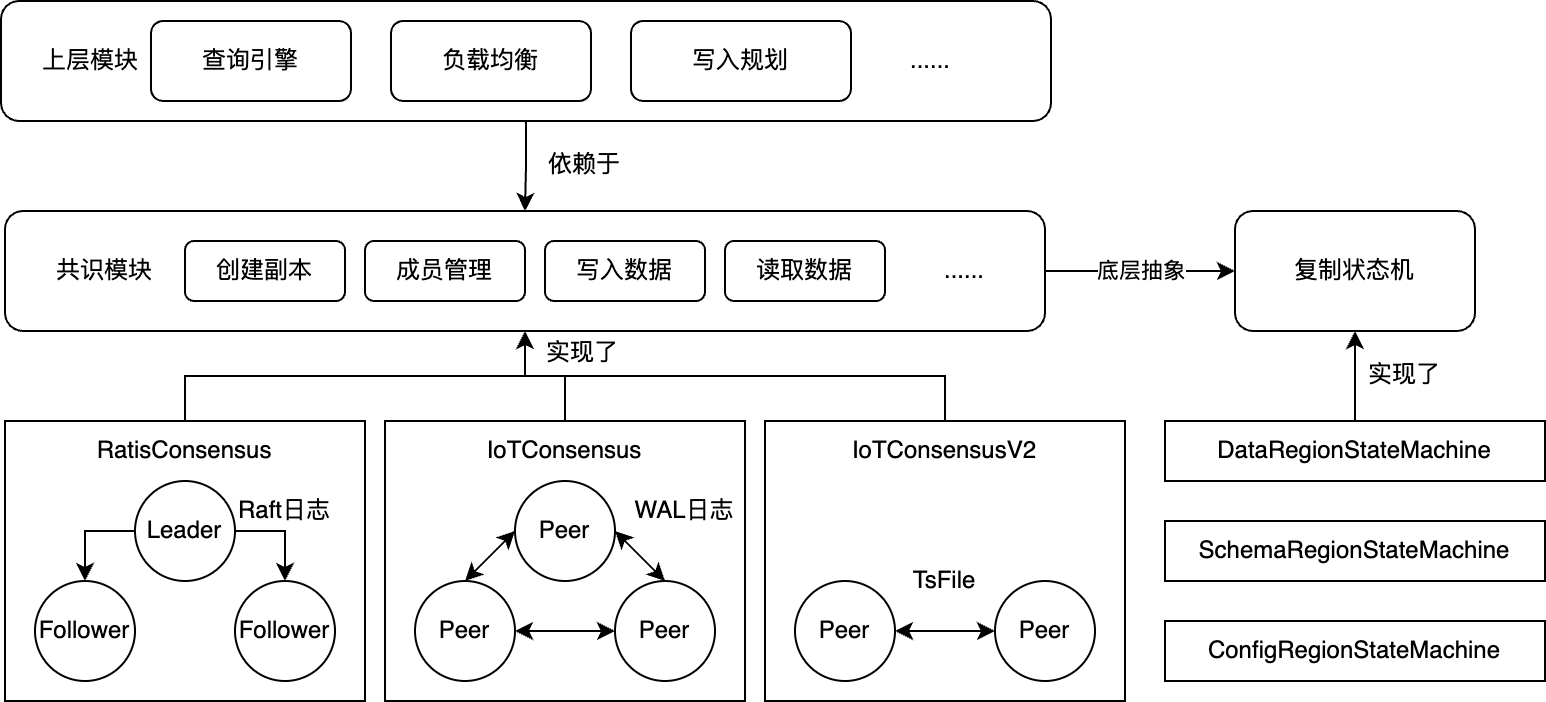
\includegraphics[width=0.99\linewidth]{c04-consensus-arch.png}
    \caption{共识层统一框架架构图}
    \label{fig:c04-consensus-arch}
  \end{figure}
  
图\ref{fig:c04-consensus-arch} 给出共识模块统一框架的示意图。

共识模块要求所有的上层服务遵循复制状态机(replicated state machine)\cite{lamport1978statemachine}的规范。目前,实现复制状态机规范的包括存储引擎(DataRegionStateMachine),元数据存储引擎(SchemaRegionStateMachine)和集群分区和管理服务(ConfigRegionStateMachine)。

共识模块定义针对数据副本组的标准接口,包括创建和销毁数据副本、在数据副本上执行写入操作、从数据副本中读取数据、对数据副本的数量、组成成员进行变更等能力。

目前IoTDB中实现了共识模块标准接口的共识协议有三种,分别是基于Raft算法的强一致性共识协议RatisConsensus,基于多主复制的会话一致性共识协议IoTConsensus和基于主从快照同步的最终一致性共识协议IoTConsensusV2。

\subsection{强一致性共识实现RatisConsensus}

RatisConsensus是IoTDB提供的强一致性共识协议实现,基于Raft共识算法和Apache Ratis\cite{ratis}开源项目实现。由于RatisConsensus提供强一致性的语义保障,目前已成为集群元数据管理和管理节点分区服务默认的共识协议。

RatisConsensus内部会维护奇数(2n+1,默认为3)个副本,并为每一个副本提供强一致性的语义保障。由于底层依赖的Raft算法是基于单主复制结构的共识协议,因此在任何时刻,这些副本中只有一个可以接受上层的写入请求,被称为领导者副本,剩下节点从领导者副本同步数据,可以接受只读请求。
RatisConsensus能够自动容忍少数副本的失效,依然保持数据和服务的可用性。具体来说,对于一个2n+1副本的RatisConsensus服务,最多能够容忍n个副本的失效。同时,RatisConsensus能够保证在网络分区情况下的数据一致性,同一时刻能保证最多只有一个副本成为领导者副本。
当领导者副本失效之后,RatisConsensus内部存在自动\failover 的机制,通过新一轮的内部选举在短时间内(默认4-8秒)选出一个新的领导者副本。

RatisConsensus底层的一致性协议是Raft算法,包含领导者选举、日志复制和安全性保障等核心要素。Raft通过随机超时来实现领导者选举,通过任期(Term)来保证每次选举的唯一性和权威性。领导者接受写入数据,并将自身日志强制复制给所有Follower,最终所有的日志可以被排列出一个副本之间达成共识的全序序列,不同的副本均按照这个全序序列应用日志,从而实现副本数据之间的一致性。为确保安全性,Raft 引入 Commit 机制,即只有在大多数副本上保存对应日志条目后,该日志才能被 Commit,上层才能收到共识层写入成功的回应。

\begin{figure}
  \centering
  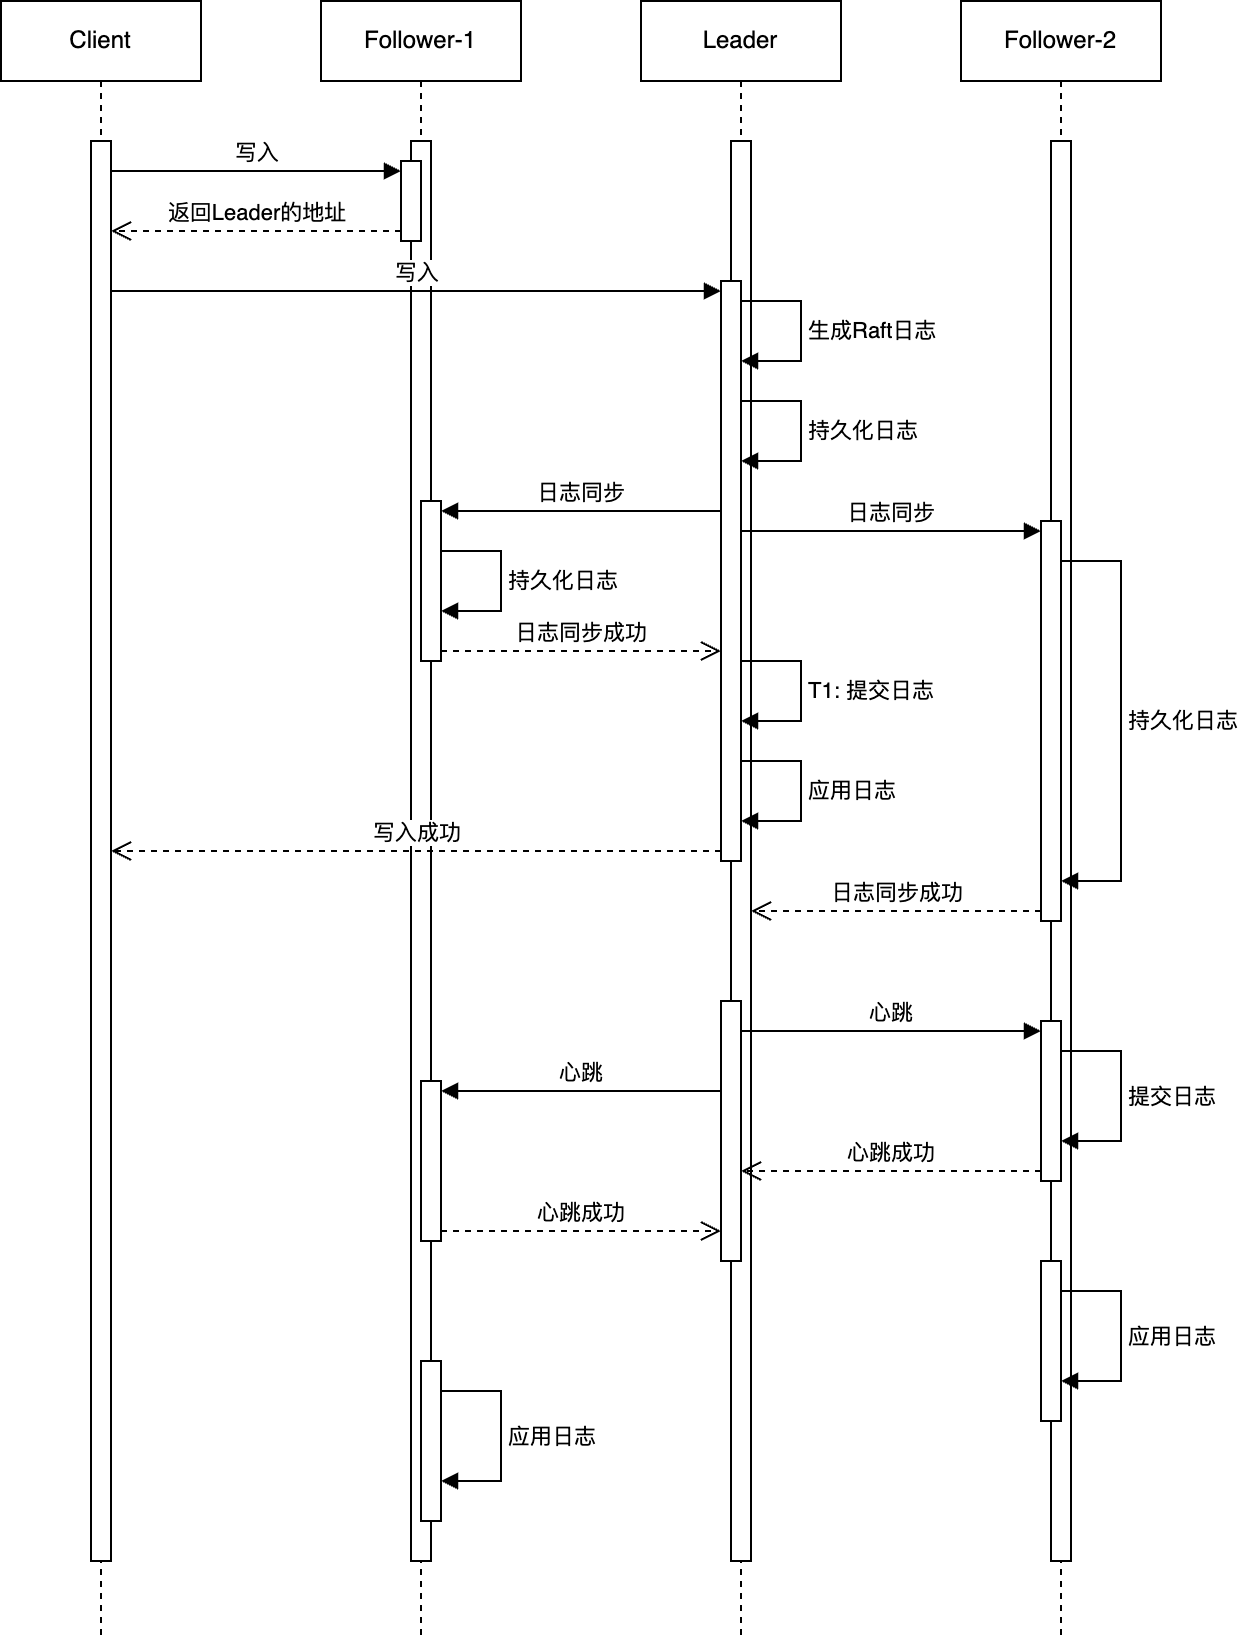
\includegraphics[width=0.7\linewidth]{c04-ratis-write.drawio.png}
  \caption{RatisConsensus数据写入和副本复制流程}
  \label{fig:c04-ratis-write}
\end{figure}

图\ref{fig:c04-ratis-write}给出一条数据提交给RatisConsensus之后背后的数据复制流程。用户写入数据之后,会由领导者这边负责生成持久化日志并同步到所有节点上,在T1时刻,有超过半数的节点完成持久化同步之后,该操作的状态将会改变成Commit,领导者会应用这个日志并返回对应的结果。Raft算法会在后台保证所有节点能够最终都Commit并应用这个日志。



\subsection{会话一致性共识实现IoTConsensus}

IoTConsensus是IoTDB提供的会话一致性共识协议实现,基于多主异步复制的自研实现,针对工业物联网时序场景写入模式有针对性的优化。目前,IoTConsensus是集群数据管理的可选共识协议之一。

IoTConsensus的设计初衷是为牺牲一定的可用性换取极致的可用性和更高的性能。
用于在工业物联网场景中,设备不断的时序数据,每台设备的写入请求往
往是串行无重复的,因而并发的写入请求之间通常不存在冲突。因此,IoTConsensus放宽了串行化的一致性约束,允许任何一个副本都能接受读写请求,并且请求在一个副本上执行成功即可返回客户端操作成功。


\begin{figure}
  \centering
  \subcaptionbox{IoTConsensus整体结构\label{fig:c04-iot-arch}}
    {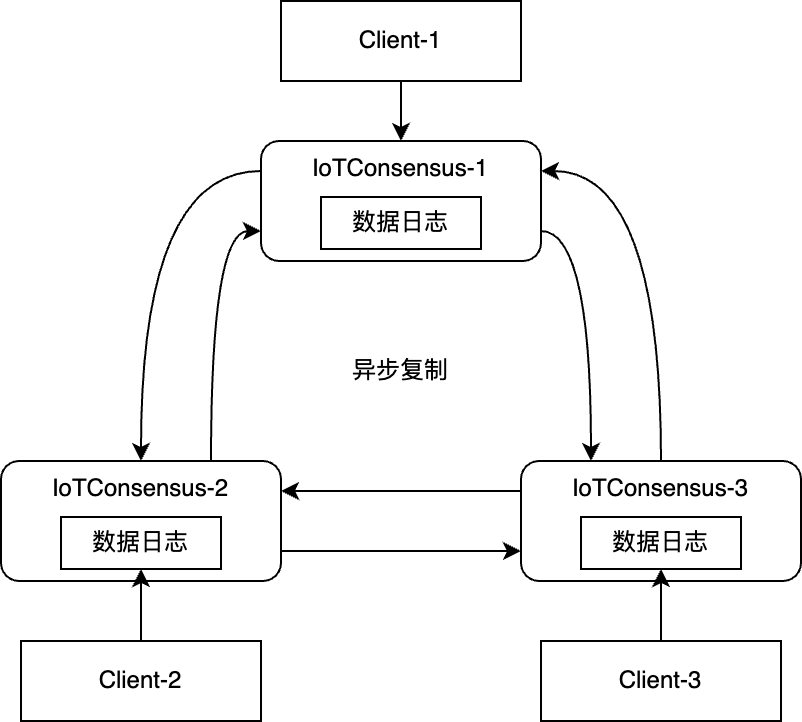
\includegraphics[width=0.4\linewidth]{c04-iot-arch.png}}
  \subcaptionbox{IoTConsensus写入流程\label{fig:c04-iot-write}}
    {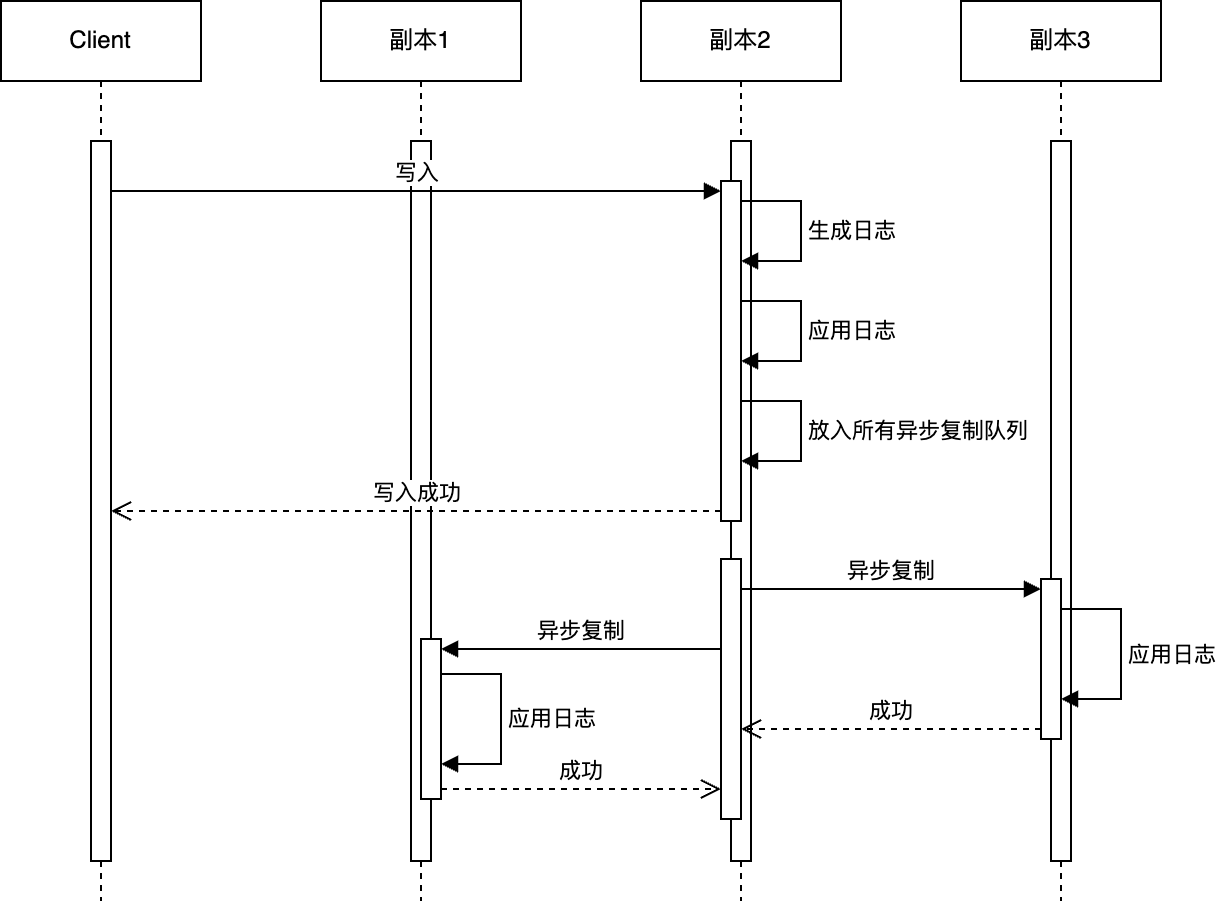
\includegraphics[width=0.58\linewidth]{c04-iot-write.png}}
  \caption{IoTConsensus示意图}
  \label{fig:c04-iot-consensus}
\end{figure}

图\ref{fig:c04-iot-arch}展示了IoTConsensus的结构,允许任何一个副本接受客户端的写入请求,并通过每个节点的后台异步复制线程将写入请求通过WAL的方式同步给其他的副本。


值得注意的是,当不同副本的数据产生冲突时,可能会导致副本之间数据无法达到最终一致,该问题的解决需要应用层的介入。例如在 Apache IoTDB 中,如果观察到某个序列的数据在不同副本上不一致,则可以使用 Select Into 子句拉取该序列在当前领导者副本上的数据并
重新向该共识组流式写入。但在绝大部分的正常应用场景,这种不一致不会发生。

虽然IoTConsensus支持多个副本的同时并发写入,但在实践过程中,为了提高性能、降低并发冲突,管理节点会为IoTConsensus挑选一个名义意义上的“主副本”,并默认将所有的写入请求引导到这个副本上。当“主副本”发生故障时,管理节点会启动故障容错和恢复机制,推举一个新的副本成为名义“主副本”。


\subsection{最终一致性共识实现IoTConsensusV2}

IoTConsensusV2是IoTDB提供的最终一致性共识协议实现,基于主从异步复制的自研实现,针对工业物联网时序场景写入模式有针对性的优化。目前,IoTConsensusV2是集群数据管理的可选共识协议之一。

IoTConsensusV2相较于IoTConsensus相比,进一步牺牲了副本之间的同步时延、一致性级别,换取了极高的写入吞吐。IoTConsensusV2的总体思路是允许在部分场景下使用TsFile进行副本间的数据同步。基于TsFile的同步过程仅涉及到常数级别的复杂度操作,同时不用经过 WAL 的磁盘持久化和 MemTable 的内存维护,因此写入吞吐非常高,并且能够解决IoTConsensus存在的由于Follower宕机或领导者节点写入速率大于同步速率导致的WAL文件堆积和写入阻塞的问题。

然而,TsFile的生成相比每一条写入日志需要较长的时间,副本间数据同步延迟在极端环境下可达到几十分钟甚至是几个小时。在两副本的情况下,如果主副本宕机,可能出现由于部分数据还未同步导致的数据暂时丢失的情况。如果宕机节点后续永久没有加入集群,那么这部分数据就会永久丢失。

\begin{figure}
    \centering
    \includegraphics[width=0.8\linewidth]{c04-pipe-consensus.redraw2.png}
    \caption{IoTConsensusV2的整体结构}
    \label{fig:c04-pipe-consensus}
  \end{figure}
  
图\ref{fig:c04-pipe-consensus}给出了IoTConsensusV2的整体架构。IoTConsensusV2具备以下两种同步模式:

1. Stream传输模式。在默认状态下使用WAL进行数据同步,来达到更快的同步速度和更高的一致性。当WAL堆积或者TsFile堆积的场景下,切换到TsFile进行数据传输,来达到更低的资源消耗和并提高吞吐。

2. Batch传输模式。该模式下,所有的数据同步都通过TsFile实现。

和IoTConsensus相似,管理节点也会为IoTConsensusV2挑选一个名义意义上的“主副本”,并默认将所有的写入请求引导到这个请求上。当“主副本”发生故障时,管理节点会启动故障容错和恢复机制,推举一个新的副本成为名义上的“主副本”。


\subsection{不同共识实现对比}

下表给出了共识模块中三个共识协议的对比。

\begin{table}
    \centering
    \caption{共识协议对比}
    \begin{tabular}{cccc}
      \toprule
      特性         & RatisConsensus & IoTConsensus &  IoTConsensusV2 \\
      \midrule
      副本一致性级别   & 线性一致性 & 会话一致性 &  最终一致性 \\
       副本复制策略    & 半同步    & 异步       & 异步       \\
       自动\failover     &  内部选举    &  管理节点指定    & 管理节点指定  \\ 
      共识协议结构   & 主从 & 多主 &  多主  \\
      数据同步性能   & 一般 & 较高 &  极高  \\
      \bottomrule
    \end{tabular}
    \label{tab:consensus-compare}
  \end{table}


\section{分布式系统高可用实践研究}

\subsection{Cassandra系统的高可用方案}
Cassandra\cite{lakshman2010cassandra}是一个开源的分布式NoSQL数据存储系统,用于管理分布在大量廉价服务器上的海量结构化数据,具备水平可扩展性、灵活的数据模型、无单点故障的高可用性等优点。

\subsubsection{Cassandra系统整体架构}

\begin{figure}
  \centering
  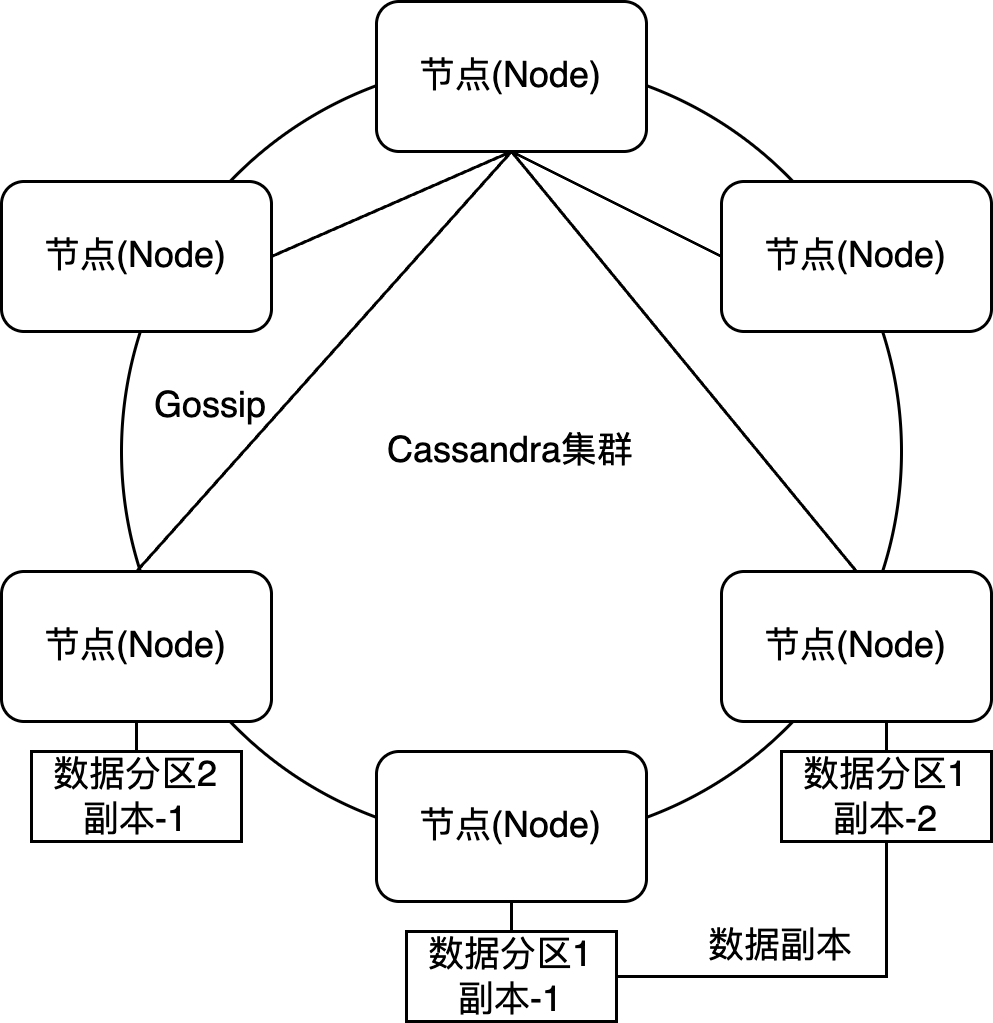
\includegraphics[width=0.6\linewidth]{cassandra-arch.png}
  \caption{Cassandra系统整体架构图}
  \label{fig:cassandra-arch}
\end{figure}

Cassandra的基本组成单元是节点,节点代表单个运行Cassandra进程的实例,通常运行在成本较低的商用硬件上。

Cassandra集群通常由多个节点组成。每个节点是同质性的,都具备独立处理客户端读写请求的能力,任何一个节点都可以作为客户端请求的协调者,负责将请求转发给存储相关数据的其他节点。节点是Cassandra线性可扩展性的基础,通过增加节点进行横向扩展,Cassandra可以增加其管理的数据量、服务的吞吐量。

Cassandra 使用基于环的数据分布方式。集群中的节点在逻辑上组织成一个环状结构 。数据会被进一步划分为更小粒度的分区,通过一致性哈希算法\cite{karger1997consistent}分布在环上的各个节点中。每个节点被分配到环上的一段 token 范围,并负责存储和管理该范围内的所有数据。

\subsubsection{数据复制和共识协议}


Cassandra通过数据副本来保证可用性和容错能力,通过一致性协议保证副本的一致性。

Cassandra通过复制因子为同一个分区保留多个副本,保证即使一个副本宕机,其他副本仍然可以满足请求。副本可以被放置在不同的数据中心,从而获得更高的安全性和性能。

Cassandra通过一致性级别来决定操作的一致性,表示在操作被视为成功之前,必须向协调器确认读取或写入操作的最小Cassandra节点数。例如,在三个副本的情况下,用户可以将一致性级别设置为1/2/3,分别代表副本写入至少1/2/3个节点之后才能确认写入操作成功。除了指定具体的副本数,用户还可以将一致性设置为QUORUM,此级别要求大多数的副本节点成功确认写入操作;也可以将一致性级别设置成为ALL,这是最强的一致性级别,要求所有的副本节点都必须成功确认写入操作。

根据Cassandra 的官方文档和普遍实践,默认的一致性级别是1,因此写入操作只需要一个副本确认即可返回。这为Cassandra集群提供了最终一致性的保障。

\subsubsection{节点故障检测}\label{sec:cassandra-failure-detecttion}

Cassandra中的每个节点通过Gossip协议来定期交换彼此的信息,并使用Phi累积性故障(Phi Accrual)检测算法\cite{hayashibara2004spl}来判断某个节点是否出现故障。

每个节点定期(通常每秒一次)通过Gossip协议选择几个其他节点交换彼此的状态信息,包括节点的运行状态、负载信息、该节点已知集群中其他节点的信息,使得信息可以快速有效地传播到整个集群。Gossip协议是一种最终一致性协议,通过这种去中心化的方式,随着时间的推移,所有节点最终都会收敛到一致的集群状态。

Cassandra中的每个节点都在本地维护着一个故障检测器,采用Phi累积性故障检测算法来标记故障节点。故障检测器会根据 Gossip 协议接收到的其他节点的状态信息和历史记录,通过统计分析心跳间隔,来预测节点失效的概率,判断集群中的其他节点是否已经宕机或者已经从故障中恢复。这种机制会综合考虑网络的性能、节点的工作负载以及历史的运行状况,从而更准确地判断节点是否真正发生故障。用户可以通过调整$phi\_convict\_threshold$属性来控制故障检测器的灵敏度。较低的值会增加将无响应节点标记为宕机的可能性,而较高的值则会降低这种可能性,适用于网络环境不太稳定的场景。


\subsubsection{故障的容错和转移}

当客户端向 Cassandra 集群写入数据时,协调器节点会根据复制策略将写入操作发送给相应的副本节点。如果某个目标副本节点由于网络问题、硬件故障或其他原因而不可用时,协调器节点会将本次写入操作的相关信息(即“提示”)存储在本地。等到宕机的节点恢复并重新加入集群时,协调器节点会检测到该节点的恢复,并将之前存储的提示转发给该节点,从而确保数据能够最终被写入到所有应该存储的副本上,实现数据的最终一致性。
提示信息中包含了目标宕机节点的位置、版本元数据以及实际需要写入的数据。
提示信息默认会在协调器节点上保存 3 小时,这个时间可以通过配置参数 $max\_hint\_window\_in\_ms$ 进行调整。


\subsection{TiDB系统的高可用方案}
TiDB\cite{huang2020tidb}是开源的分布式关系性数据库,同时支持OLTP和OLAP的能力,具备水平扩缩容、金融级高可用、实时 HTAP、云原生、兼容MySQL生态等优势。

\subsubsection{TiDB的整体架构}

TiDB集群可以划分为位于中间代理层的TiProxy,位于计算层的TiDB,位于存储层的TiKV和TiFlash以及集群的协调节点PD(Placement Driver)。

\begin{figure}
  \centering
  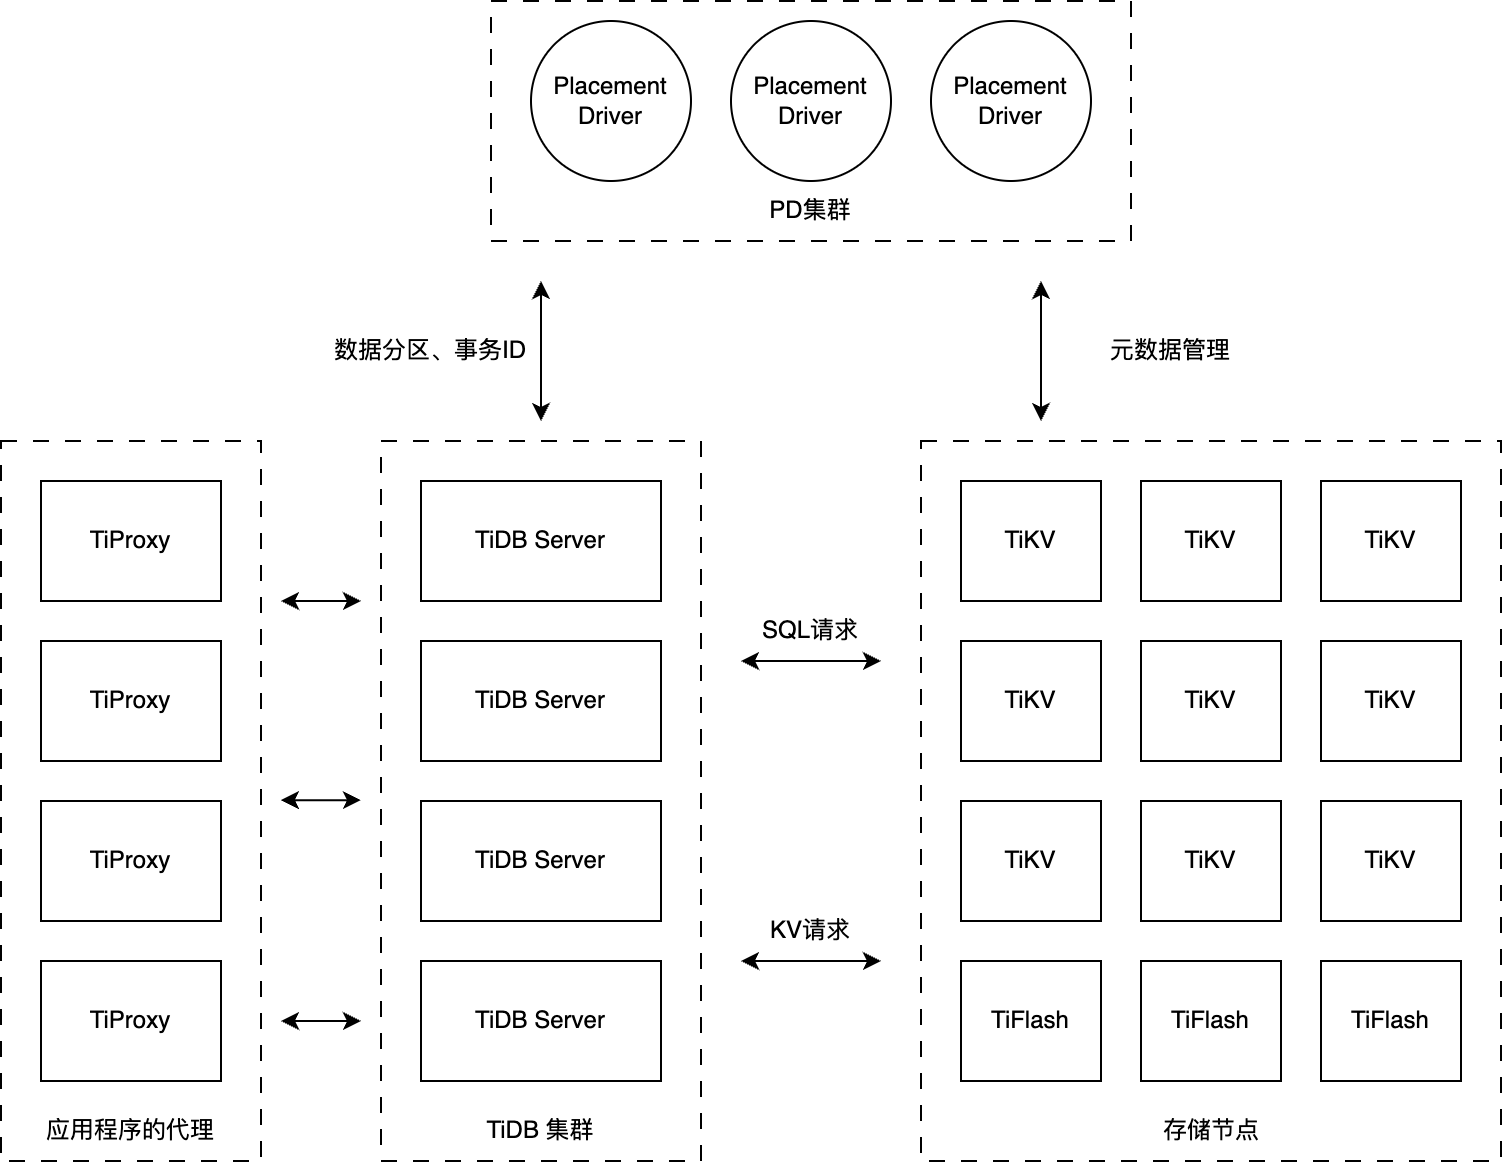
\includegraphics[width=0.9\linewidth]{related-tidb-arch.png}
  \caption{TiDB系统整体架构图}
  \label{fig:tidb-arch}
\end{figure}

PD是集群的管理服务,负责集群元数据、节点和数据分区的管理、监控和调整。PD使用Raft协议来保证自身的高可用和元数据的一致性。

TiKV和TiFlash是数据的存储节点。TiKV是具备分布式事务能力的键值存储引擎,而TiFlash是为查询负载专门优化的列式存储引擎。数据的存储以分区作为单位,包含了一段Key的区间,TiKV通过分区来实现数据分区和负载均衡,并会为每一个分区维护多个副本来保证高可用性,TiDB使用Raft作为副本的一致性协议。

TiDB是无状态的计算节点,在接收到来自客户端的连接之后,对传入的 SQL 语句进行解析和优化,并最终生成分布式执行计划,并将计划转发给存储节点执行。

TiProxy是部署在客户端应用和TiDB之间的代理节点,提供负载均衡、连接持久化、服务发现和其他功能。


\subsubsection{故障的检测和发现}

在TiDB集群中,PD负责对存储节点TiKV进行故障检测,TiProxy负责对TiDB进行故障检测。

TiKV会定期向PD发送心跳包,交换的内容包括总磁盘容量和磁盘用量、节点承载的分区数量、数据写入和读取的负载情况、发送/接收的snapshot数量等相关信息。如果PD在一段时间内没有收到TiKV的心跳,那么就会认为该节点可能出现故障,将其状态标记为异常,并且综合考虑用户配置和集群实际情况,来判断是否将该节点从集群中移除,并进行相应的调度操作,例如将该TiKV上的分区进行迁移。每一个分区的Raft领导者也会定期向PD发送心跳包,交换的内容包括领导者所在的位置、每一个Follower所在的位置、掉线的副本个数和该分区的写入/读取速度。当领导者掉线,其他的Follower节点可能会触发新的选举,同时若PD长时间没有收到心跳,也可能触发主动的领导者切换和副本的调度。


TiProxy会通过定期的健康检查来测试TiDB节点的状况。TiProxy会尝试模拟一个客户端连接,并执行一个非常轻量级的操作,如果连接成功建立并在规定的超时时间内完成操作,该TiDB就通过了健康检查。如果某个 TiDB 实例未能通过健康检查,负载均衡器就会停止向该实例转发流量,从而有效地将故障的 TiDB 实例隔离。



\subsubsection{故障的转移和恢复}

当PD检测到TiKV发生故障后,会启动主动的\failover 流程。首先,故障节点上的Raft领导者会在超时之后变得不可用,其他节点上的Follower副本会检测到这一超时并主动展开选举。同时,PD 还会将故障节点上的副本数据调度到其他的TiKV节点上进行复制以恢复到预期的副本数量,保障数据的冗余性。

PD节点的故障则通过Raft主动的领导者选举机制进行容错,只要集群中超过半数的 PD 节点是可用的,PD 集群就能继续正常工作。

由于 TiDB Server 是无状态的,单个或多个 TiDB Server 实例的故障不会导致数据丢失。前端的负载均衡器会通过健康检查机制检测到故障的 TiDB Server,并停止向其转发流量,而是将请求转发给其他健康的 TiDB Server 实例。为了应对故障或增加处理能力,可以很容易地向集群中添加新的 TiDB Server 实例。

上述策略保证了系统整体的RPO为零,RTO为分钟级。


\subsection{OceanBase系统的高可用方案}

OceanBase是开源的分布式关系性数据库,兼具分布式架构的扩展性和集中式架构的性能优势,通过单一引擎支持混合事务/分析处理,具备高性能、高可用性、强一致性、水平扩展性和兼容SQL生态等优势。

\subsubsection{OceanBase的整体架构}

OceanBase集群主要包括OBServer和OBProxy两个角色。每一个OBServer上都运行着OceanBase的一个进程,内部可进一步细分为根服务、SQL引擎、事务引擎和存储引擎。OBProxy则充当中间层,接收来自应用程序的SQL请求,将其路由到集群内最佳的OBServer节点,然后将执行结果返回给应用程序。

\begin{figure}
  \centering
  \includegraphics[width=0.8\linewidth]{related-OceanBase-arch.png}
  \caption{OceanBase系统整体架构图}
  \label{fig:OceanBase-arch}
\end{figure}

根服务是集成在OceanBase进程内的逻辑服务,负责维护集群的元数据,包括表结构、分区信息、节点状态等。根服务会通过心跳机制检测每一个OBServer的健康状况,如果发现故障,则会触发恢复流程,包括重新选举领导者或重新复制分区。根服务还会负责监控集群的负载情况,会进行分区移动、分区复制和领导者切换等操作以确保各个节点的资源利用率均衡。

OBServer还包含了SQL引擎,用于接收用户请求并生成对应的计划,以及基于LSM结构的存储引擎。

集群内的元数据和用户数据都是以分区的方式进行水平划分和存储,并通过副本复制的方式保证分区的高可用。OceanBase采用了基于哈希和范围的双层划分算法,但会保证同一个表组的分区被分配在同一个节点上。OceanBase采用Paxos算法对每一个分区的重做日志进行复制管理,在故障恢复时,通过重放重做日志实现恢复。

OBProxy 用于将请求路由到 OBServer。当接收到用户的 SQL 查询时,OBProxy 将解析该查询,然后根据分区的位置信息将查询发送到相应的 OBServer,提供服务发现和负载均衡等能力。


\subsubsection{副本复制}

OceanBase 采用多副本机制来实现数据冗余,每个分区通常拥有三个副本,这些副本分布在不同的机房,以实现灾难恢复。OceanBase 采用基于 Paxos 协议的同步复制模型以确保跨副本的数据强一致性。数据复制是通过日志流机制实现的。领导者副本上写入操作产生的重做日志会被复制到 Follower 副本 。Follower 副本会实时回放这些重做日志,以保持与领导者副本的一致性 。


\subsubsection{OceanBase的故障检测优化}

OceanBase通过校验和、使用单独的健康检测通道、基于RPC机制的节点检测等方式,尽可能提前发现故障的时间。

在校验和上,OceanBase在每次从磁盘中读写数据的时候都会计算和比较校验和,在每次大合并之后对每一个数据分区的副本重新比对校验和,在重放重做日志的时候会计算每一条事务的累积校验和。通过事务粒度的校验和机制,OceanBase能够发现软件实现中事务处理和并发控制两个模块的人为程序漏洞。

在单独的健康监测通道上,OBProxy通过RPC请求的返回状态对OBServer进行存活判断,这种判断方式可能在队列请求积压或者整个节点负载升高的时候出现误判,导致 OBProxy 误把一个正常服务的节点标记在黑名单。因此,OBProxy会和节点建立一条单独的探测连接,只用于节点的存活分析,避免写入读取请求积压对健康探测的影响。

在基于RPC机制的节点检测上,OceanBase 4.0中,节点间健康状态监测机制从基于TCP的连接机制转变为基于RPC框架内部的方式。3.0版本中OceanBase采用定期发送TCP Keepalive的探测包来检测节点之间的网络连接是否正常,然而这种检测只能用于判断网络情况,如果OBServer进程出现问题(例如Coredump崩溃),但TCP连接依然存在,KeepAlive机制无法识别。因此,在4.0版本中,OceanBase框架内置了健康状态监测机制,通过定期发送应用程序级别的心跳包,从而能同时监测网络和进程的健康状态。同时,由于RPC 框架内部的检测机制能够检测应用程序的响应延迟、错误率等指标,从而提供更细粒度的健康状态信息。



\subsubsection{OceanBase的故障恢复}

OceanBase通过大幅减少故障单元、对Paxos并行回放、加快Paxos领导选举流程等方式提高故障恢复的速度。

在前文所提到的TiDB中,故障恢复单元颗粒度是每一个Raft组。当上层业务的分区特别多、单一节点上承载的Raft组数量特别多的情况下,故障恢复的单元数量就会水平扩张,量级巨大。因此,在OceanBase 4.0版本之后,故障恢复的单元被优化成一个单机的日志流,在逻辑上可以把每一个节点视作一个整体的Paxos组,因此故障恢复单元将不再和业务的元数据和实际数据量有关,从而进一步降低了故障恢复的复杂性和时间。

同时,为了提高故障恢复的速度,OceanBase需要进行并行、实时地回放日志中的事务,从而防止日志回放成为性能的瓶颈。在OceanBase中,不同事务的重做日志可以并行回放,同一事务的不同重做日志也可以并行回放,通过事务的ID来保证并发的安全性。

在Paxos选举优化上,传统的Paxos选举流程基于随机算法,并且依赖节点之间的时钟同步,例如NTP协议。OceanBase的实现消除了对节点间时钟同步的依赖,完全基于消息驱动,依靠节点之间的消息交互和顺序来触发选举,并激进地将领导者的Lease时间缩短到了4s以内,从而能够更快地检测到故障并完成新的领导者选举。同时,当集群检测到节点故障时,对于领导者副本在这个节点上的Paxos组,根服务会直接指定组内的其他Follower副本展开选举,跳过随机心跳超时,在百毫秒的级别就把服务切换到一个新的副本上。这种方式有助于加速故障的恢复,减少总的RTO时间。


\subsection{TDengine系统的高可用方案}

TDengine 是一款开源的时间序列数据库,为物联网数据、工业监控和大数据分析而设计。它针对海量时间序列数据进行了优化,具备高写入速率和低查询延迟的特性。

\subsubsection{TDEngine的架构}

TDEngine采用分布式架构,在集群中存在以下关键的逻辑单元:

1.管理节点:管理节点负责元数据的管理、监控数据节点的状态以及协调集群操作。为了提高可靠性,一个 TDengine 集群最多可以配置 3 个管理节点。

2.数据节点:集群的核心处理单元,负责存储和管理时间序列数据。每个数据节点可以托管多个虚拟节点。

3. 虚拟节点:虚拟节点是数据节点内的虚拟存储单元,用于保存数据采集点的时间序列数据和元数据。来自单个数据采集点的数据始终存储在同一个虚拟节点上。

4. 查询节点:查询节点负责处理查询操作,可以与虚拟节点位于同一个数据节点上,也可以在不同的数据节点上运行,从而实现存储和计算的分离。

TDengine使用多数据副本和Raft算法来维护副本的一致性。位于不同数据节点上相同数据的虚拟节点的不同副本组成的逻辑单元是虚拟节点组,通过 Raft 一致性算法进行同步,其副本数量可以在创建数据库时通过参数进行配置。为了实现高可用性,副本数量应大于 1,并且数据节点的数量必须至少等于副本数量。 


\subsubsection{TDengine的故障检测}

TDengine采用多方面的方法进行故障检测,结合了通过心跳进行的主动监控和通过专用工具对系统指标进行的被动观察。

数据节点和管理节点在集群内会定期通过心跳通信其状态,管理节点通过心跳机制来监控数据节点的健康状况和虚拟节点组内的节点跟踪领导者状态。虚拟节点组内的节点也会相互交换Raft心跳,确定每个成员的状态,如果跟随者节点在一定的选举超时时间内没有收到心跳,则会发起新一轮的领导者选举。

此外,TDengine还会通过监控工具对集群健康状态监测。taosKeeper会收集和导出 TDengine集群的监控指标,将这些指标写入一个独立的 TDengine 实例,从而实现独立的监控。这些监控指标最后会被可视化到Grafana面板TDinsight上,包含集群状态、节点信息(数据节点、管理节点、虚拟节点)、请求统计和资源使用情况(CPU、内存、磁盘)。它还能够监控数据节点和管理节点的存活率。


\subsubsection{\failover 和故障恢复}

TDengine依赖Raft的选举机制进行故障恢复。
数据节点上,每个虚拟节点组内,Raft 一致性算法确保,如果领导者虚拟节点发生故障,将自动从跟随者节点中选举出一个新的领导者。此过程确保数据访问的中断控制在选举超时的时间内。
管理节点上,TDengine支持配置多个管理节点,以实现元数据管理服务的高可用性。Raft协议也用于维护管理节点之间的一致性,如果领导者管理节点发生故障,跟随者节点可以接管。

对于故障下线的节点来说,如果节点离线时间少于 给定的阈值,它会自动重新加入集群,通过预写日志和自动从其他在虚拟节点组中的副本重新同步数据的方式来恢复服务。



\section{本章小结}

本章回顾了分布式系统故障处理以及高可用性与容错领域的相关研究工作。
本章首先深入探讨了分布式系统中故障的普遍性、根本原因、不同分类以及由此带来的挑战,并明确了本研究关注的典型故障场景。
其次,详细阐述了高可用与容错的核心概念、衡量指标(如SLA、RTO、RPO)以及关键技术,包括数据复制、共识协议(如Paxos、Raft)、故障检测、\failover 、自动恢复(日志与检查点)和主动式容错策略(如负载均衡)。
接着,本章阐述了Apache IoTDB的高可用性和容错能力的现有建设:共识模块,包含共识的统一框架和三种一致性不同的实现RatisConsensus、IoTConsensus、IoTConsensusV2.
最后,为了借鉴成熟系统的实践经验,本章对 Cassandra、TiDB、OceanBase和TDengine 四个业界的分布式数据库系统的高可用架构、故障检测机制及恢复策略进行了剖析,表格\ref{tab:ha-comparison}给出了Apache Cassandra、TiDB、OceanBase和TDEngine四个分布式数据库系统在高可用能力方面的比较。这些对现有理论、技术和工业实践的梳理与分析,为本文后续针对 Apache IoTDB 提出的高可用优化方案提供了重要的理论依据和实践参考。


\begin{table}[h!]
  \centering
  \caption{不同系统之间的高可用和容错能力的比较}
  \label{tab:ha-comparison}
  \begin{tabular}{@{}lllll@{}}
      \toprule
      比较指标 & Cassandra & TiDB & OceanBase & TDengine\\
      \midrule
      数据副本 & 多副本 & 多副本 & 多副本 & 多副本 \\
      一致性 & 最终一致性 & 强一致性 & 强一致性 & 强一致性\\
      共识算法 & 冲突修复 & Raft & Paxos & Raft\\
      故障检测 & 心跳+Phi检测& 心跳超时 & 心跳超时+RPC连接 & 心跳超时 \\
      \failover &向副本转移& 等待主副本恢复 & 等待主副本恢复 & 等待主副本恢复 \\
      故障恢复 &协调者同步 & Raft主副本同步 & Paxos日志同步 & Raft主副本同步\\
      RPO & 0 & 0 & 0  & 0\\
      RTO & 分钟级& 分钟级 & 秒级 & 分钟级\\
      \bottomrule
  \end{tabular}
\end{table}